 
% header.tex
\documentclass[a4paper,11pt,twoside,ngerman,color]{book}
\usepackage[a4paper,left=3.5cm,right=2.5cm,bottom=3.5cm,top=3cm]{geometry}


% Korrekte Darstellung der Umlaute
\usepackage[utf8]{inputenc}
\usepackage[T1]{fontenc}

\usepackage[ngerman]{babel}
\usepackage[autostyle]{csquotes}
\usepackage[]{dirtytalk}

\usepackage[pdftex]{graphicx,color}
\definecolor{LightGray}{RGB}{211, 211, 211}

\usepackage{amsmath,amssymb,subcaption}%,subfigure

\usepackage{calc}
\usepackage{tikz}
\usetikzlibrary{positioning,calc,arrows,shapes.multipart,arrows.meta}

\usepackage[altpo, epsilon]{backnaur}
\renewcommand{\bnfpn}[1]{\textbf{\textrm{#1}}}
\renewcommand{\bnfsp}[0]{,}
\renewcommand{\bnfts}[1]{\textquotedbl\texttt{#1}\textquotedbl}
\newcommand{\bnfop}[1]{[ #1 ]}
\newcommand{\bnfre}[1]{\{ #1 \}}
%\renewcommand{\bnfpn}[1]{\textbf{\textrm{#1}}}
%\renewcommand{\bnfts}[1]{\bnf@tsfont{#1}}

% Theorem-Umgebungen
\usepackage[amsmath,thmmarks]{ntheorem}

% Algorithmen
\usepackage[plain,chapter]{algorithm}
\usepackage{algorithmic}

% Listings
\usepackage{minted}
\usepackage{listings}
\lstdefinestyle{customprometheus}{
	belowcaptionskip=1\baselineskip,
	breaklines=true,
	frame=L,
	numbers=left,
	xleftmargin=\parindent,
	language=C,
	showstringspaces=false,
	stepnumber=1,
	basicstyle=\footnotesize\ttfamily,
	keywordstyle=\bfseries\color{green!40!black},
	commentstyle=\itshape\color{purple!40!black},
	identifierstyle=\color{blue},
	stringstyle=\color{orange},
}

\newmintinline[promcode]{text}{fontsize=\scriptsize, bgcolor=LightGray}


\makeatletter
\let\footnote@orig\footnote
\def\footnote{%
	\begingroup
	\@makeother\#%
	\footnote@i
}
\def\footnote@i#1{%
	\endgroup
	\footnote@orig{#1}%
}
\makeatother


\usepackage{enumerate}


% Bibtex deutsch
%\usepackage{bibgerm}
\usepackage[
backend=biber,
%style=authoryear-icomp,
style=numeric-comp,
sortlocale=de_DE,
natbib=true,
%url=false, 
%doi=true,
%eprint=false
]{biblatex}
\addbibresource{literatur/diplom.bib}

\usepackage[]{hyperref}
\hypersetup{
	%colorlinks=true,
	hidelinks
}

% URLs
\usepackage{url}

% Abbr
\usepackage{glossaries}
\makeindex

\newglossaryentry{latex}
{
        name=latex,
        description={Is a mark up language specially suited for 
scientific documents}
}

\newglossaryentry{maths}
{
        name=mathematics,
        description={Mathematics is what mathematicians do}
}

\newglossaryentry{formula}
{
        name=formula,
        description={A mathematical expression}
}

\newacronym{iot}{IoT}{Internet of things}
\newacronym{pql}{PQL}{Prometheus Query Language}
\newacronym{tsdb}{TSDB}{Time Series Database}
\newacronym{promql}{PromQL}{Prometheus Query Language}
\newacronym{bzgl}{bzgl.}{bezüglich}
\newacronym{IP}{IP}{Internet Protocol}
\newacronym{IPv4}{IPv4}{Internet Protocol version 4}
\newacronym{IPv6}{IPv6}{Internet Protocol version 6}
\newacronym{ip-address}{IP-address}{Internet Protocol Address}
\newacronym{http}{HTTP}{Hyper Text Transfer Protocol}
\newacronym{ebnf}{EBNF}{Extended Backus–Naur form}
\newacronym{json}{JSON}{JavaScript Object Notation}
\newacronym{tudortmund}{TU Dortmund}{Technische Universität Dortmund}
\newacronym{ide}{IDE}{integrated development environment}
\newacronym{dsl}{DSL}{domain specific language}
\newacronym{mgl}{MGL}{meta graph language}
\newacronym{msl}{MSL}{meta style language}
\newacronym{w}{W}{Watt}
\newacronym{percent}{\%}{percent}
\newacronym{degreeC}{$^\circ$C}{degree celcius}
\newacronym{url}{URL}{Uniform Resource Locator}
\newacronym{ui}{UI}{User Interface}
\newacronym{emf}{EMF}{Eclipse Modeling Framework}
\newacronym{uml}{UML}{Unified Modeling Language}

% Caption Packet
\usepackage[margin=0pt,font=small,labelfont=bf]{caption}
% Gliederung einstellen
%\setcounter{secnumdepth}{5}
%\setcounter{tocdepth}{5}

% Theorem-Optionen %
\theoremseparator{.}
\theoremstyle{change}
\newtheorem{theorem}{Theorem}[section]
\newtheorem{satz}[theorem]{Satz}
\newtheorem{lemma}[theorem]{Lemma}
\newtheorem{korollar}[theorem]{Korollar}
\newtheorem{proposition}[theorem]{Proposition}
% Ohne Numerierung
\theoremstyle{nonumberplain}
\renewtheorem{theorem*}{Theorem}
\renewtheorem{satz*}{Satz}
\renewtheorem{lemma*}{Lemma}
\renewtheorem{korollar*}{Korollar}
\renewtheorem{proposition*}{Proposition}
% Definitionen mit \upshape
\theorembodyfont{\upshape}
\theoremstyle{change}
\newtheorem{definition}[theorem]{Definition}
\theoremstyle{nonumberplain}
\renewtheorem{definition*}{Definition}
% Kursive Schrift
\theoremheaderfont{\itshape}
\newtheorem{notation}{Notation}
\newtheorem{konvention}{Konvention}
\newtheorem{bezeichnung}{Bezeichnung}
\theoremsymbol{\ensuremath{\Box}}
\newtheorem{beweis}{Beweis}
\theoremsymbol{}
\theoremstyle{change}
\theoremheaderfont{\bfseries}
\newtheorem{bemerkung}[theorem]{Bemerkung}
\newtheorem{beobachtung}[theorem]{Beobachtung}
\newtheorem{beispiel}[theorem]{Beispiel}
\newtheorem{problem}{Problem}
\theoremstyle{nonumberplain}
\renewtheorem{bemerkung*}{Bemerkung}
\renewtheorem{beispiel*}{Beispiel}
\renewtheorem{problem*}{Problem}

% Algorithmen anpassen %
\renewcommand{\algorithmicrequire}{\textit{Eingabe:}}
\renewcommand{\algorithmicensure}{\textit{Ausgabe:}}
\floatname{algorithm}{Algorithmus}
\renewcommand{\listalgorithmname}{Algorithmenverzeichnis}
\renewcommand{\algorithmiccomment}[1]{\color{grau}{// #1}}

% Zeilenabstand einstellen %
\renewcommand{\baselinestretch}{1.25}
% Floating-Umgebungen anpassen %
\renewcommand{\topfraction}{0.9}
\renewcommand{\bottomfraction}{0.8}
% Abkuerzungen richtig formatieren %
\usepackage{xspace}
\newcommand{\vgl}{vgl.\@\xspace} 
\newcommand{\zB}{z.\nolinebreak[4]\hspace{0.125em}\nolinebreak[4]B.\@\xspace}
\newcommand{\bzw}{bzw.\@\xspace}
\newcommand{\dahe}{d.\nolinebreak[4]\hspace{0.125em}h.\nolinebreak[4]\@\xspace}
\newcommand{\etc}{etc.\@\xspace}
\newcommand{\evtl}{evtl.\@\xspace}
\newcommand{\ggf}{ggf.\@\xspace}
\newcommand{\bzgl}{bzgl.\@\xspace}
\newcommand{\so}{s.\nolinebreak[4]\hspace{0.125em}\nolinebreak[4]o.\@\xspace}
\newcommand{\iA}{i.\nolinebreak[4]\hspace{0.125em}\nolinebreak[4]A.\@\xspace}
\newcommand{\sa}{s.\nolinebreak[4]\hspace{0.125em}\nolinebreak[4]a.\@\xspace}
\newcommand{\su}{s.\nolinebreak[4]\hspace{0.125em}\nolinebreak[4]u.\@\xspace}
\newcommand{\ua}{u.\nolinebreak[4]\hspace{0.125em}\nolinebreak[4]a.\@\xspace}
\newcommand{\og}{o.\nolinebreak[4]\hspace{0.125em}\nolinebreak[4]g.\@\xspace}
\newcommand{\oBdA}{o.\nolinebreak[4]\hspace{0.125em}\nolinebreak[4]B.\nolinebreak[4]\hspace{0.125em}d.\nolinebreak[4]\hspace{0.125em}A.\@\xspace}
\newcommand{\OBdA}{O.\nolinebreak[4]\hspace{0.125em}\nolinebreak[4]B.\nolinebreak[4]\hspace{0.125em}d.\nolinebreak[4]\hspace{0.125em}A.\@\xspace}

% Leere Seite ohne Seitennummer, naechste Seite rechts
\newcommand{\blankpage}{
	\clearpage{\pagestyle{empty}\cleardoublepage}
}

% Keine einzelnen Zeilen beim Anfang eines Abschnitts (Schusterjungen)
\clubpenalty = 10000
% Keine einzelnen Zeilen am Ende eines Abschnitts (Hurenkinder)
\widowpenalty = 10000 \displaywidowpenalty = 10000
% EOF



\begin{document}
	\selectlanguage{ngerman}
	\begin{titlepage}
\definecolor{TUGreen}{rgb}{0.517,0.721,0.094}
\vspace*{-2cm}
\newlength{\links}
\setlength{\links}{-1.5cm}
\sffamily
\hspace*{\links}
\begin{minipage}{12.5cm}

\includegraphics[width=8cm]{bilder/tud_logo_rgb}
%\hspace*{-0.25cm} \textbf{TECHNISCHE UNIVERSITäT DORTMUND}\\
%\hspace*{-1.2cm} \rule{5mm}{5mm} \hspace*{0.1cm} FACHBEREICH INFORMATIK\\
\end{minipage}

\vspace*{4cm}

\hspace*{\links}
\hspace*{-0.2cm}
\begin{minipage}{9cm}
\large
\begin{center}
{\Large Bachelorarbeit} \\
\vspace*{1cm}
\textbf{Modelgetriebene Sensordatenverarbeitung / Model-driven Sensor Data Processing} \\
\vspace*{1cm}
Dennis Ochocki\\
% \vspace*{1cm}
März
\end{center}
\end{minipage}
\normalsize
\vspace*{5.5cm}

% \hspace*{\links}

\vspace*{2.1cm}

\hspace*{\links}
\begin{minipage}[b]{5cm}
% \normalsize
\raggedright
Gutachter: \\
Prof. Dr. Bernhard Steffen \\
Tim Tegeler \\
\end{minipage}

\vspace*{2.5cm}
\hspace*{\links}
\begin{minipage}[b]{8cm}
% \normalsize
\raggedright
Technische Universität Dortmund \\
Fakultät für Informatik\\
Lehrstuhl für Programmiersysteme (5)\\
http://ls5-www.cs.tu-dortmund.de
\end{minipage}
%%%%%%%%%%%%%%%%%%%%%%%%%%%%%%%%%%%%%%%%%%%%%%%%%%
% bei Kooperation mit anderen Lehrstuehlen,
% sonst weglassen
% \begin{minipage}[b]{8cm}
% \normalsize
% \raggedleft
% In Kooperation mit:\\
% Fakultätsname\\
% Lehrstuhl-/Institutsbezeichnung
% \end{minipage}
%%%%%%%%%%%%%%%%%%%%%%%%%%%%%%%%%%%%%%%%%%%%%%%%%%

\end{titlepage}

	\blankpage
	\pagenumbering{roman}
	\tableofcontents
	\cleardoublepage
	\pagenumbering{arabic}
	% Kapitel
	% einleitung.tex
\chapter{Introduction}
As the digitization proceeds over time it is important to not get overwhelmed by the complexity growing. \gls{it} assistance is the counterpart guiding and helping society to master the difficulty of this development. To ensure that processes and devices are working and doing what they should, regular measurement and periodic observation are indispensable. In case of failure it provides the necessary information for fixing the problematic situation or even prevent them in the first place. Build in sensors can be found inside many devices, which can be fundamental for correct functionality. For example engines in cars need sensors to work as desired. Furthermore common devices like a fridge or an electric oven has thermometers since they need to know how much and when to cool down or heat up. 

The smart home is a topic becoming more established in the consumer market. It is getting easier to set up a network of smart home components where room temperature or humidity is tracked, the light can be controlled from the smartphone and the heating is shutting down at night. Configurations can be done through web interfaces and the already available wireless network at home is used for their communication.

For managing and observing those networks a variety of tools can be used. Most of the smart home sensor devices have proprietary interfaces allowing to only work in a closed system from one manufacturer. Fortunately some devices are able to interconnect with others from various manufacturers. 

\section{Motivation and Background}
Since the complexity rises with the size of the sensor network it is advising to abstract these network and try to create a structure with could help to keep track of it. Not only measuring a handful of devices but every power socket or thermostat in a building and using their values in a reasonable manner is difficult to achieve. It is not only the size of the network but using various different devices and all their varying metrics is another challenge to master. To make non computer scientists able to create such networks a well designed tool is needed that reduces the complexity. Architects or other experts in room design and life quality could then easily create sensor systems without coding.

\section{Structure of the Work}
As the work is based on Prometheus, Grafana and Cinco a brief introduction in each topic will be given in \autoref{chapter:grundlagen}. Afterwards in \autoref{chapter:bestandsaufnahme} the first ideas of an abstraction from a real world scenario will be created. Additionally a model and all needed constraints will be developed. Using the results from previous steps in \autoref{chapter:realisierung} an implementation in Cinco will be done. Furthermore, the model will be modified were it is needed to get the implementation work the right way. Additionally an example will show how working with the generated \gls{ide} looks like. At last in \autoref{chapter:conclusion} a summary will be added, arisen problems will be discussed and final thoughts will be included in an outlook.
\clearpage
% kapitel2.tex
\chapter{Preliminaries}
\label{chapter:grundlagen}
Because the thesis covers many different systems each of them has to be introduces at least at a decent level. Modern and best of breed solution are being used here. Grafana and Prometheus are software products as a optional additional setup in cluster systems like kubernetes to monitor their technical values. As a little bonus and for easier developing process docker and docker compose will be used but in a very simple way. That technologies form the target of the \gls{dsl} designed in this thesis. For the realization of the \gls{dsl} and compiler Cinco, a meta modeling tool will be used.
 
\section{Smart Home}
In the course of digitalization and simplification of the procurement of sensor technology in everyday life, smart home has arrived as a concept for the consumer and is affordable. In the most general case, it is a base station with any number of actuators and sensors. This station is used to process and store the data from the sensory elements of the network and the actuators act on the basis of decision tables, for example. As a simple scenario, one can imagine a living room lamp that is switched on when the brightness sensor outside signals darkness. However, a system does not necessarily has to have sensors and actuators. A network of sensors would only monitor and one of actuators can only act. Examples would be a central power consumption monitoring per socket or a remote light control.
Here it is worth mentioning that there are also crossover devices. A heating thermostat usually has a built-in thermometer and is thus both actuator and sensor.\todo{add 1-2 par}\\

\begin{figure}[!h]
	\centering
	\begin{tikzpicture}[every text node part/.style={align=center}]
	\node[] (A) {
\includegraphics[width=50px]{./assets/images/plug-solid}\\sensor};
	\node[right= 3cm of A] (B) {
\includegraphics[width=50px]{./assets/images/chalkboard-solid}\\base station};
	\node[right= 3cm of B] (C) {
\includegraphics[width=50px]{./assets/images/lightbulb-solid}\\actuator};
	\draw[-{Stealth[scale=1.3,angle'=90]},semithick] (B) -- node[above] {0..N} (A) ;
	\draw[-{Stealth[scale=1.3,angle'=90]},semithick] (B) -- node[above] {0..M} (C) ;
	\end{tikzpicture}
	\caption{Abstract Smart Home Network}
\end{figure}
\todo{add source of images}
\section{Basic Terms}
In the context of Prometheus and this thesis, a few potentially ambiguous terms need to be specified more precisely.
\subsection{Metric}
A property which is observed and measured.
\begin{Beispiel}
	Temperature, rain amount, brightness, transfer rate, amount of printed documents
\end{Beispiel}
\begin{Definition}
	A metric is a single property to be measured.
\end{Definition}
\subsection{Sensor}
A sensor is a real device, a unit which is used in the real world. This can capture multiple metrics and then make them available via an interface.
\begin{Beispiel}
	Weather station, network switch, heating thermostat
\end{Beispiel}
\begin{Definition}
	A metric is a single property to be measured.
\end{Definition}

\section{Prometheus}
Prometheus is an open source solution that is used for metrics monitoring and alerting. There is the possibility to pass data actively or alternatively to configure Prometheus to fetch data from different data sources. For the latter variant, the system to be monitored must provide an \gls{http} interface on which the data is delivered in a predefined manner. Finally the collected data is persisted on the internal time series database.

To simplify this process, there are already several libraries for different programming languages that are configurable to export such a format. At the time of writing GO, Scala/Java, Python and Ruby are officially supported, but for many other languages there are unofficial third party libraries which are advertised on the Prometheus website. 

In case the selected language is not supported, it is also possible to create the output yourself. For this, the definition of the output format has been well documented.
\subsection{Metric Types}
Prometheus distinguishes between different types of metrics. In the following, all possibilities are briefly explained. In the \autoref{subsec:Exportformat} for understanding a few examples listed and explained.
\subsubsection{Counter}
The counter describes a metric type which can only be incremented and reset. It represents a monotonically growing function. 
\subsubsection{Gauge}
This type symbolizes a speedometer. The values can rise and fall.
\subsubsection{Histogram}
A histogram is a concept consisting of so-called buckets. These are initially defined for a metric. With the help of this definition, values of $]-\infty,+\infty[$ are sorted into the said buckets. Each next higher bucket also contains the measured values of the lower bucket. So it is a subset relation where the subsets are determined by the set limit. The \promcode{le} in the index can be interpreted as \textquote{Less Equal}. This parameter is also noted like this in the export.
\begin{figure}[htp!]
	\begin{tikzpicture}
	\draw (0,0) ellipse (2cm and .7cm);
	\draw (2,0) ellipse (4cm and 1cm);
	\draw (4,0) ellipse (6cm and 1.3cm);
	\draw (6,0) ellipse (8cm and 1.5cm);
	\path (0,0) -- (12,0)%
	node[pos=0] {$B_{le=``0.1''}$}%
	node[pos=0.33] {$B_{le=``0.5''}$}%
	node[pos=0.66] {$B_{le=``1''}$}%
	node[pos=1] {$B_{le=``+Inf''}$};
	\end{tikzpicture}
	\caption{Relation of Bucket in a Histogram}
\end{figure}
A histogram represents, in addition to the buckets, a total number of measured values, which is like a bucket with \promcode{le="+Inf"} and a value for the sum of all values.
\begin{figure}[hbt!]
	\begin{minted}[mathescape,
	linenos,
	numbersep=5pt,
	gobble=0,
	frame=lines,
	linenos,
	tabsize=4,
	breaklines,
	framesep=2mm]{text}
	# TYPE <basename> histogram
	<basename>_bucket{le="<upper inclusive bound>"} <value>
	<basename>_sum <value>
	<basename>_count <value>
	\end{minted}
	\caption{General Concept of a Histogram Export}
\end{figure}
Line 2 can occur multiple times as each entry hat its own limit value. Lines 3 and 4 are the additional values as already mentioned.
\subsubsection{Summary}
\begin{figure}[h!]
	\begin{minted}[mathescape,
		linenos,
		numbersep=5pt,
		gobble=0,
		frame=lines,
		linenos,
		tabsize=4,
		breaklines,
		framesep=2mm]{text}
		# TYPE <basename> histogram
		<basename>{quantile="<φ>"} <value>
		<basename>_sum <value>
		<basename>_count <value>
	\end{minted}
	\caption{General Concept of a Summary Export}
\end{figure}
A summary is similar to a histogram, but here buckets are not filled by the value of the measurement but the measured values are divided into $\varphi$-quantiles ($0 \le \varphi \le 1)$ and the maximum value of the quantile.
\subsubsection{Untyped}
In this case a value is assigned to the metric without following any special rules. This is a safe default setting and it is inevitable not to use this type.
\Needspace{9\baselineskip}
\subsection{Labels}
Labels can be used to break down metrics with the same name into different origins. 
\begin{figure}[!ht]
	\begin{minted}[mathescape,linenos,numbersep=5pt,gobble=1,frame=lines,tabsize=4,breaklines,framesep=2mm]{text}
	<basename>{key="<value>",key2="<value2>",...} <value>
	\end{minted}
	\caption{General Concept of Labels}
\end{figure}
\subsection{Exportformat}
\label{subsec:Exportformat}
The export format of Prometheus can be described well by means of an example. For this purpose, we draw a part from the official documentation~\cite{PrometheusExpositionFormatBeispiel}.\\
\par
\begin{listing}[H]
	\begin{minted}[mathescape,linenos,numbersep=5pt,gobble=0,frame=lines,linenos,tabsize=4,breaklines,framesep=2mm]{text}
	# HELP http_requests_total The total number of HTTP requests.
	# TYPE http_requests_total counter
	http_requests_total{method="post",code="200"} 1027 1395066363000
	http_requests_total{method="post",code="400"}    3 1395066363000
	
	# Minimalistic line:
	metric_without_timestamp_and_labels 12.47
	\end{minted}
	\caption{Partial Example from the Official Prometheus Documentation~\cite{PrometheusExpositionFormatBeispiel}}
\end{listing}
Between lines 1-4 we find the first exported metric in this example. The first line contains after the token \promcode{# HELP <name of metric>} a short description which is Optional. The next line specifies the type with \linebreak \promcode{# TYPE <name of metric> <type of metric>}. The choices regarding the type coincide with the metric types already described: \promcode{counter}, \promcode{gauge}, \promcode{histogram}, \promcode{summary}, \promcode{untyped}.

All lines starting with \promcode{#} but not continued with \promcode{TYPE} or \promcode{HELP} are comment lines and therefore not interpreted.

Lines 3-4 show the measured values broken down by their labels. Lines that symbolize the measured values consist of three columns. The first in the format \promcode{<name of metric>} followed by optional labels in curly brackets. The example here breaks down all \gls{http} requests by method and \gls{http} return value. The next column contains the measured value for the metric, taking into account the optional grouping available. The last column is again non-mandatory and contains the timestamp at which the value was measured. 
In addition, we have a minimal example in line 7. Due to the lack of type specification, the type is \promcode{untyped}. The \gls{ebnf} to this type of line is as follows:
\begin{listing}[H]
	\begin{samepage}
		\begin{minted}[mathescape,
		linenos,
		numbersep=5pt,
		gobble=1,
		frame=lines,
		linenos,
		tabsize=4,
		breaklines,
		framesep=2mm]{ebnf}
		metric = metric_name, [ 
		"{",
		label_name, "=", '"', label_value, '"',
		{ ",", label_name, "=", '"', label_value, '"' }, [ "," ], 
		"}",
		],  value,  [ timestamp ];
		\end{minted}
		\caption{\gls{ebnf} following ISO/IEC 14977 of a Metric}
	\end{samepage}
\end{listing}

In the following lines you can see a more complex example. This is a histogram. The values measured internally in the exporter are divided into so-called buckets. You can see the four preconfigured buckets with the limits \promcode{0.05}, \promcode{0.2}, \promcode{1} and \promcode{+Inf}. 
\begin{listing}[H]
	\begin{minted}[mathescape,linenos,numbersep=5pt,gobble=1,frame=lines,tabsize=4,breaklines,framesep=2mm]{text}
	# HELP http_request_duration_seconds A histogram of the request duration
	# TYPE http_request_duration_seconds histogram
	http_request_duration_seconds_bucket{le="0.05"} 24054
	http_request_duration_seconds_bucket{le="0.2"} 100392
	http_request_duration_seconds_bucket{le="1"} 133988
	http_request_duration_seconds_bucket{le="+Inf"} 144320
	http_request_duration_seconds_sum 53423
	http_request_duration_seconds_count 144320
	\end{minted}
	\caption{Histogram Export Example from the Official Prometheus Documentation~\cite{PrometheusExpositionFormatBeispiel}}
\end{listing}
\todo{mention summary?}

\subsection{Prometheus Query Language}
As mentioned before, the collected data is stored in an internal Time Series database \todo{never mentioned} which can be searched by the so-called \gls{promql}.

There are four different subtypes for this:
\subsubsection{Instant vector}
Instant vector selectors allow the selection of a set of time series and a single sample value for each at a given timestamp (instant). In the simplest form, only a metric name is specified. This results in an instant vector containing elements for all time series that have this metric name. \todo{semantik der typen beschreiben}

\section{Grafana}
\label{sec:grafana}
For the visualization of the data collected by Prometheus, Grafana~\citep{GrafanaHomepage} can be used. It is a versatile and extensible system to display data from various data sources like databases like Cassandra, MariaDB or PostgreSQL but also regular \gls{http} requests against external interfaces or static \gls{json} objects are possible~\cite{GrafanaDataSources}. Furthermore, Grafana also provides different types of diagrams.
\todo{better layout, following fig.}
\begin{figure}[ht]
	\begin{subfigure}{.25\textwidth}
		\centering
		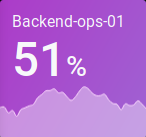
\includegraphics[width=.8\linewidth]{assets/screenshots/Screenshot_2020-12-08 1 - New Features in v7 0 - Grafana.png}
		\captionsetup{justification=centering}
		\caption{Single Metric\\with Graph}
		\label{fig:sfig1}
	\end{subfigure}%
	\begin{subfigure}{.25\textwidth}
		\centering
		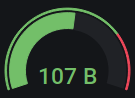
\includegraphics[width=.8\linewidth]{assets/screenshots/Screenshot_2020-12-08 Website trends - Grafana.png}
		\captionsetup{justification=centering}
		\caption{Single Metric\\as Gauge}
		\label{fig:sfig2}
	\end{subfigure}%
	\begin{subfigure}{.5\textwidth}
		\centering
		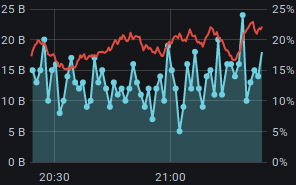
\includegraphics[width=.8\linewidth]{assets/screenshots/Screenshot_2020-12-08 Grafana Play Home - Grafana(2).png}
		\captionsetup{justification=centering}
		\caption{Multimetric plot}
		\label{fig:sfig2}
	\end{subfigure}
	\caption{Example Diagram Types in Grafana}
	\label{fig:fig}
\end{figure}
Supplementary there is a simple table format, honeycomb patterns, bar charts and many more. These, like the data sources, are extensible through plug-ins. Thanks to the source code openness of the project, custom plug-ins can be written if needed.

To fill the diagrams with data from, in our case, Prometheus, a \gls{promql} query must be stored in each diagram, which is executed regularly. Such a diagram is part of a so-called panel. That means, a panel has exactly one diagram and vice-versa. These are now combined into dashboards, which then provide an overview. Here you can define a lot of panels to display them at the same time.

It should also be said that there are higher order structures such as organizations or you can summarize dashboards again in playlists and / or groups. These features are not considered in this work however more near.

\subsection{Panels}
Since panels have many settings and thus allow many individualization, these are briefly explained here.

Each panel has primarily a name, description, diagram type, settings for the layout and value reference of cumulative functions and behavior with zero values. Depending on the selected chart type, different configurations are possible. Axis labeling, legend, limits for symbolic coloring and other specific settings.

Alternatively to the grouping of metrics, which is possible by keywords, it is a option to display several metrics in one diagram by specifying multiple \gls{promql} queries. More can be found in chapter 6: Visualization Panels In Grafana of~\cite{Salituro2020}.

\section{Model-driven development}

Generalization, classification and aggregation forms the most common form called abstraction~\cite{Brambilla_2017}. Software development cannot exist without it, as it gives the developer the ability to ignore not important properties of a real world situation. Therefore this helps breaking down the observed scene into essential parts leading to a simpler description of the given situation. As a synonym often modeling instead of abstraction is used. Based on this model, which is acquired by abstraction, a developer can now realize and implement a software which fulfills all needs and constraints expressed by the model. 

In today complex world abstraction is indispensable and helps to create models in everyday life. It is a tool to eradicate unnecessary information or properties which can not be understood today. A good example for a well known abstraction is playing billiard. Bank shots can be for example abstracted with the rule, that the angle of incidence equals the angle of reflection. This can be true for most of the shots, but taking the spin of the white ball under consideration the abstraction will not longer work. The next physical property which could be included into the model would be the elasticity of the cushions or traction on the bed. Every time information is ignored a abstraction layer is created.

Abstraction is the fundamental technique of model-driven development. Additionally it utilizes different tools and standards for visualization, notation and the development process. A very common and popular notation is the \gls{uml}~\cite{Cook2017}. Powerful tooling and development assist can be found with \gls{emf}. This framework give the ability to model in a well defined way using the meta model Ecore. It is meta as it allows to describe other models~\cite[section 2.3.1]{steinberg2008emf}. The focus is on creating a perfect model, defining all constraints and dependencies. From here the implementation is just following the abstract model, since the work of discussing and committing to a mutual objective is already done.

\gls{emf} not only contains the Ecore model, but also a generator for example for code, custom files or an customized Eclipse \gls{ide} providing support for the model.


\section{Cinco}
Everything above is a necessary base technology where on top of it the model-driven solution, the domain specific language is build. For this task the meta modeling tool Cinco~\cite{CincoHomepage} will be used. The full name is \say{CINCO SCCE Meta Tooling Framework} and it utilizes the \gls{emf} and Graphiti Graphical Tooling Infrastructure. It is in active development of the chair for programming systems of the \gls{tudortmund}.

The \gls{mgl} allows the user, like \gls{emf} already does, to design a custom \gls{dsl} and generate a working \gls{ide} with features like auto complete or code generation and additionally visual editing in the generated \gls{ide}. This is a very interesting point, because modeling a \gls{dsl} which can be used in a visual editor reduces the amount of work needed to get started with using this \gls{dsl} for non computer scientists essentially. 

Because Cinco is a meta modeling tool generating graphical \glspl{ide} it is also needed to somehow influence the visual appearance and exactly describe the style of the elements defined in the \gls{mgl} files. 

\begin{figure}
	\begin{tikzpicture}
		\path (0,0) node (eclipse) [anchor=north west,minimum width=2cm,align=center, minimum height=1.2cm, inner sep=0] {\shortstack{Eclipse\\Devs}};
		\path (0,-1.4) node (cinco) [anchor=north west,minimum width=2cm,align=center, minimum height=1.2cm] {\shortstack{Cinco\\Devs}};
		\path (0,-2.8) node (cp) [anchor=north west,minimum width=2cm,align=center, minimum height=2.4cm] {\shortstack{CP\\Devs}};
		\path (0,-5.2) node (user) [anchor=north west,minimum width=2cm,align=center, minimum height=1.2cm] {\shortstack{CP\\User}};
		\path (2,0)    node [anchor=north west,fill=blue!20,rounded corners,minimum width=\textwidth-2cm, minimum height= 1.2cm, inner sep=0] {};
		\path (2,-1.4) node [anchor=north west,fill=blue!20,rounded corners,minimum width=\textwidth-2cm, minimum height= 1.2cm, inner sep=0] {};
		\path (2,-2.8) node [anchor=north west,fill=blue!20,rounded corners,minimum width=\textwidth-2cm, minimum height= 2.2cm, inner sep=0] {};
		\path (2,-5.2) node [anchor=north west,fill=blue!20,rounded corners,minimum width=\textwidth-2cm, minimum height= 1.2cm, inner sep=0] {};
		\path (3.25,-.3) node (ecore) [anchor=north west,draw, rounded corners, minimum width=3cm, minimum height=.6cm, align=center, inner sep=0] {Ecore.ecore};
		\path (2.5,-1.7) node (cincod1) [anchor=north west,draw, rounded corners, minimum width=2.2cm, minimum height=.6cm,  align=center, inner sep=0] {MSL.ecore};
		\path (4.8,-1.7) node (cincod2) [anchor=north west,draw, rounded corners, minimum width=2.2cm, minimum height=.6cm, align=center, inner sep=0] {MGL.ecore};
		\path (8.5,-1.5) node (l) [anchor=north,draw, rounded corners, minimum width=2.5cm, minimum height=1cm, align=center, inner sep=0] {\footnotesize\shortstack{Cinco Code\\Generator}};
		\path (2.5,-2.9) node [anchor=north west,draw, rounded corners, minimum width=4.5cm, minimum height=2cm, align=center, inner sep=1mm,text height=1.6cm,] {\footnotesize High-Tool Level Specification};
		
		\path (2.75,-3.2) node (devs1) [anchor=north west,draw, rounded corners, minimum width=1.5cm, minimum height=.8cm, align=center, inner sep=1mm] {\footnotesize Sensor.mgl};
		
		\path (5.05,-3.2) node (devs2) [anchor=north west,draw, rounded corners, minimum width=1.5cm, minimum height=.8cm, align=center, inner sep=1mm] {\footnotesize Sensor.msl};
		
		\path (10,-2.9) node [anchor=north west,draw, rounded corners, minimum width=4.5cm, minimum height=2cm, align=center, inner sep=0mm,text depth=1cm,] {\footnotesize\shortstack{Tool Realization\\(Cinco Product)}};
		
		\path (12.25,-3.8) node (tool) [anchor=north,draw, rounded corners, minimum width=1.5cm, minimum height=.8cm, align=center, inner sep=1mm] {\footnotesize Sensor.ecore};
		
		\path (10,-5.5) node (user1) [anchor=north west,draw, rounded corners, minimum width=2cm, align=center, inner sep=0,minimum height=.6cm] {a.sensor};
		\path (12.5,-5.5) node (user2) [anchor=north west,draw, rounded corners, minimum width=2cm, align=center, inner sep=0,minimum height=.6cm] {b.sensor};
		
		
		\draw[-{Triangle[width=18pt,length=8pt]}, line width=10pt, color=orange!20](7.1,-3.9) -- (9.9,-3.9);
		\path (8.5,-3.9) node {\Huge\color{black}\faCog};
		\path (8.5,-3.9) node (cog) {\huge\color{white}\faCog};
		\draw [dashed] (cog.west) -- (l.south west);
		\draw [dashed] (cog.east) -- (l.south east);
		\draw [-{Triangle}] (user1.north) -- (tool);
		\draw [-{Triangle}] (user2.north) -- (tool);
		\draw [-{Triangle}] (devs1.north) -- (cincod1);
		\draw [-{Triangle}] (devs2.north) -- (cincod2);
		\draw [-{Triangle}] (cincod1.north) -- (ecore);
		\draw [-{Triangle}] (cincod2.north) -- (ecore);
	\end{tikzpicture}
	\caption{Generation of an automaton modeling tool by an abstract tool specification with the
Cinco framework~\cite[figure 4]{cincoimage}}
\end{figure}

\subsection{Meta Graph Language}
Cinco uses four different elements for modeling a \gls{dsl} inside of it. The \gls{mgl}, which is used for that modeling task, defines nodes, edges, container and type elements. Having the ability of being enhanced with fields or dependencies between them they give the developer the opportunity designing a very powerful language. Basically the \gls{mgl} is like a graph with nodes and edges expanded with optional containers where a subset of the nodes and edges elements can be stored. The type node adds the ability of defining other needed types. In general there is also the feature of extending already defined types, so little adaptions can be done a a bigger level of abstraction can be implemented.

\subsubsection{Node}

A node is an unit which can have incoming and outgoing edges. It also can have different attributes and a so-called prime reference. A prime reference is a pointer to any other node, edge or container. This allows for example to make connections between different models in different files. Because Cinco is based on the \gls{emf} it is also possible to reference any other object defined in external sources. To declare a node the first token to use is \promcode{node} preceded by optional annotations and a optional \promcode{abstract} keyword. Followed by the name of the node and a declaring body wrapped in curly brackets. The body can contain definitions of attributes the node has to have, declaration of which edge types are incoming and which outgoing with optional constraints like quantities, a style option for correct visualization and a already described prime reference. An attribute starts with the keyword \promcode{attr}, like before there are other prefixes like final and unique. A type and a name are appended, optional minimal and maximal values and a default value. For the edges \promcode{incomingEdges} or \promcode{outgoingEdges} can be used with the possibility restricting the allowed edges and adding a cardinality to this declaration. Styles can be applied to the node by using the \promcode{style} keyword with a style id.
Further the last token \promcode{prime} is used for adding a prime reference to the node. It needs the referencing type and a name to be set up correctly.

\subsubsection{Edge}
Simpler constructs are edges. They are introduced using \promcode{edge} and can only contain attributes and a style. Like in the node definition annotations, abstraction flag or inheritance can be used without making cuts.

\subsubsection{Container}
Container heavily rely on the possibilities of a node. It is capable of all features of a node but being extended by the keyword \promcode{containableElements}. This makes it possible to allow specific object to be embedded inside of this container.

\subsubsection{Type}
Attributes can have different types. Cinco has therefor the following build-in datatypes:

\begin{center}
	EString | EChar | EFloat | EBoolean | EDouble | EInt | ELong | EBigInteger | EBigDecimal | EByte | EShort | EDate
\end{center}


The custom datatypes can either be enumerations or user defined types which are groups of attributes. Optional inheritance is also possible. Enums are defined by \promcode{enum} followed by a name and all possible literals. The user defined type uses the keyword \promcode{type}, a name and the list of attributes written down the same way like in the node definition.

\subsection{Meta Style Language}
\clearpage
% kapitel3.tex
\chapter{Challenge and Approach}
\label{chapter:bestandsaufnahme}
To start a proper analysis and abstraction of the problem a starting example is needed. It is important to qualify the rules which describe how the system is build and realize the dependencies. Furthermore, because of the importance of \gls{promql} in this project it will be a big part of the analysis and model.
\section{Examples}
Because it is already known which software to use this section will be split into smaller sections for the sake of clarity. 

\subsection{Real World Situation}
In this section the properties of the system that are observable in the real world are considered closer. Sensors come in different shapes and varieties. For example single metric sensors, like thermometer, brightness sensors or power consumption. 

Additionally there are also more complex ones. Multi metric sensors for example are digital weather stations, network components like a switch or router, server metrics and so on. A specific property, which only real world sensors can have, is a location. They can be in the living room or an office building. If the whole sensor network is between multiple cities and multiple with a humidity sensor on each floor in every room it can become rather large in scale.

Summarized it is a real world gadget which provide at least one metric and is somehow bound to a location.

\subsection{Digital World}
Because the sensors are more intelligent devices in this context they have to be accessible through network via \gls{IPv4} or \gls{IPv6} and expose the metrics in a predefined syntax ( see section \ref{subsec:Exportformat}, page \pageref{subsec:Exportformat} ). 

This is the bridge to the consuming parts of the system. In the next step Prometheus is configured to actively pull the exposed metrics of the sensors in a predefined frequency. It is the possible for the sensors to push their metrics to Prometheus, but it would cause the sensors have to be configured knowing  Prometheus \gls{ip-address}. The way of pushing the data into Prometheus won't be examined further.

Since Prometheus only acts as the database, Grafana is used as a visualization toolkit. Grafana connects directly to Prometheus and uses \gls{promql} to gather information from the database storage. The possibilities mentioned in \autoref{sec:grafana} are configurable. 

Both settings for Prometheus and Grafana can be delivered with a simple configuration file, meaning there is no need to go through the setup process. 
In addition a Dockerfile will take care of the correct packaging and runtime accessibility of all needed files. Therefore this whole structure makes allows to get a single output which is capable of running Prometheus and Grafana, configured in the predefined way and already knowing the set up sensor devices.

\begin{figure}
	\centering
	\begin{tikzpicture}[n/.style={draw,thick,circle,inner sep=0pt,minimum width=1cm}]
		\node [n, label=humidity] (M1) {$M_1$};
		\node [n, below = 1cm of M1, label=temperature] (M2) {$M_2$};
		\node [n, below = 1cm of M2, label=air pressure] (M3) {$M_3$};
		\node [n, right = 2cm of M1, label=weather station] (S1) {$S_1$};
		\draw [->] (M1) -- (S1) (M2) -| ($ (M2) !.5! (S1) $) |- (S1) (M3) -| ($ (M3) !.5! (S1) $) |- (S1);
		\node [n, below = 1cm of S1] (S2) {$S_2$};
		\node [n, below = 1cm of S2] (S3) {$S_3$};
		\node [n, right = 3cm of S2, label=Prometheus] (P) {$P$};
		\draw [->] (S1) -- (P);
		\draw [->](S2) -- (P);
		\draw [->] (S3) -- (P);
		\node [n, right = 2cm of P, label=Grafana] (G) {$G$};
		\draw [->] (P) -- (G);
	\end{tikzpicture}
	\caption{Example of a Small Monitoring System}
	\label{fig:system}
\end{figure}

\begin{samepage}
\section{Abstraction}
\label{sec:abstraction}
In the abstraction layer the same approach can be used. First the real world situation has to be modeled and then the digital components.

\subsection{Real World Abstraction}

As mentioned earlier a sensor can be anything and is a physical device which measures all kinds of metrics. A simple model can be visualized in the following way:

\begin{figure}[h!]
	\centering
	\begin{tikzpicture}[n/.style={draw,thick,circle,inner sep=0pt,minimum width=1cm}]
		\node [n,inner sep=1mm] (M1) {$Metric$};
		\node [n,inner sep=1mm, left = 4cm of M1] (S1) {$Sensor$};
		\path [] 
		(S1) edge node[above, pos=0.85] {1..n} node[above, pos=0.15] {1..n} (M1);
	\end{tikzpicture}
	\caption{Abstract Model of a Sensordevice}
\end{figure}
\end{samepage}
\noindent
As shown a sensor can have 1\dots n metrics.

\subsection{Digital World Abstraction}

The transition of the digital situation into a abstract model is very linear and simple. Like in image \ref{fig:system} Grafana knows Prometheus which crawls the data of the sensors.

\begin{samepage}
\begin{figure}[h!]
	\centering
	\begin{tikzpicture}[n/.style={draw,thick,circle,inner sep=0pt,minimum width=1cm}]
		\node [n,inner sep=1mm] (S1) {$Sensor$};
		\node [n,inner sep=1mm, left = 3cm of S1] (P1) {$Prometheus$};
		\node [n,inner sep=1mm, left = 3cm of P1] (G1) {$Grafana$};
		\path [] 
			(G1) edge node[above, pos=0.85] {1} node[above, pos=0.15] {1} (P1)
			(P1) edge node[above, pos=0.85] {1..n} node[above, pos=0.15] {1} (S1)
			;
	\end{tikzpicture}
	\caption{Abstract Model of the Digital Components}
\end{figure}
\end{samepage}

The simple abstraction above shows the technical dependency and the data flow. Yet it does not consider every property which is configurable in Prometheus and Grafana. Furthermore it overlooks the meta information coming from the real world setting.

\subsection{Specification}
The abstraction in \autoref{sec:abstraction} is very basic and fundamental. Since there are more variables to take care of the model has to be extended. Due to the variety of the sensors and no option of a central management all additional configurations are done in Prometheus or Grafana.

\subsubsection{Location}
A location information is missing. Technically it can be added in each entry of the sensor in the Prometheus configuration as an additional label which will then be added as a keyword in the exported metrics. 

\begin{listing}[H]
	\begin{minted}[mathescape,linenos,numbersep=5pt,gobble=0,frame=lines,tabsize=4,breaklines,framesep=2mm]{yaml}
- job_name: '«sensor.name»'
  static_configs:
  - targets: ['«sensor.url»']
    labels:
      location: '«sensor.location»'
	\end{minted}
	\caption{Generic Sensor Configuration for Prometheus~\cite{PrometheusExpositionFormatBeispiel}}
\end{listing}

\subsubsection{Grouping of sensors}
To have a better management experience a grouping for the sensors should be introduced. It would be possible to group them via labels or metric name but this could lead to a not fully understandable networking. 

\begin{samepage}
	\begin{figure}[h!]
		\centering
		\begin{tikzpicture}[n/.style={draw,thick,circle,inner sep=0pt,minimum width=1cm}]
			\node [n,inner sep=1mm] (S1) {$sensor$};
			\node [n,inner sep=1mm, left = 3cm of S1] (P1) {$sensor group$};
			\path [] 
			(P1) edge node[above, pos=0.85] {1..n} node[above, pos=0.15] {1..n} (S1)
			;
		\end{tikzpicture}
		\caption{Abstract Model of Sensor Grouping}
	\end{figure}
\end{samepage}


\subsubsection{Prometheus Query Language}
Since one goal of this thesis is to create an abstract model of all needed configurations in Prometheus and Grafana, \gls{promql} is one important thing to be considered. Modeling a \gls{promql} query should also be possible. Vector aggregation, set operations and so on are features to be covered. 


\section{Model}

Building a \gls{dsl} on top of the previous considerations leads to a well designed model. The explanations start bottom-up which equals the development process for the user of the created \gls{dsl}. For a better overview a separation of all informational layers is needed.

The elemental components are the measurable metrics. They have a simple name and an optional unit like \gls{w}, \gls{degreeC} or \gls{percent}. A subset of the defined metrics are part of a sensor.

In the next layer the sensors are instantiated, connected with a location and combined with a handful of properties. A name and a \gls{url} of the sensor is essential. This information is needed for the configuration generation for the Prometheus service, allowing it to pull the sensor date frequently and save it in the internal database. On top, allowing an easier management sensor groups are introduced, combining multiple sensors into one node. Therefore this layer serves the spatial allocation. 

After modeling the real world situation the next layer models the Grafana service. The available sensors and sensor groups can now be used in a \gls{promql} $GraphQuery$ node. This node form the base data set for additional query selections. Technically \gls{promql} allows a high variety of different queries but for the sake of less complexity a single application of a aggregation function is allowed. Additionally \gls{promql} queries can take information for features like resolution, time window or offset. 

The defined queries can now be bundled in different Grafana panels allowing to share these queries between panels. A panel has a visualization type and matching settings for example for highest value of an axis, linear or logarithmic grid, colors or special rules for single values. No matter the type every panel has a width, height, x- and y- position based on the Grafana \gls{ui} system. This information allows to manage the panels inside a dashboard, which is the last node type of the Grafana layer. It consists of a name and a unique short string identifier which is needed for Grafana. 

Last but not least the project layer is more of the business and controlling view. The only node existing here is the project node. It can contain different meta variables welding useful information for further execution of the project like address, company name, deployment type or important \glspl{IP} addresses. 

In retrospective the model is mostly linear, leaving a straight forward way of working with the \gls{dsl} implementing this model. The separation into the four layers help the developer or engineer to think in well defined domains. They symbolize the steps of defining the used sensors, placing and grouping them in the real world and setting up the visualization for Grafana. Like already said the last layer is only used for meta data concerning the project itself.

\begin{figure}[!tb]
	\centering
	\begin{tikzpicture}[ state/.style={draw,minimum height=\ht\strutbox+\dp\strutbox, inner ysep=0pt}, label/.style={minimum height=\ht\strutbox+\dp\strutbox, inner ysep=0pt}]
		
		\node[] (bb1) {$\textbf{Layers:}$};
		\node[below=of bb1] (bb2) {$\textbf{Submodel:}$};
		\node[label, right=of bb1] (b1) {Sensor};
		\node[label, right=2cm of b1] (b2) {Floor};
		\node[label, right=2cm of b2] (b3) {Grafana};
		\node[label, right=2cm of b3] (b4) {Project};
		%\path[] (b1) edge (b2) (b2) edge (b3) (b3) edge (b4);
		
		\node[state, below=of b1] (a1) {Metrics};
		\node[state, below=of a1] (a2) {Sensor};
		\node[state, below=of b2] (aa3) {Location};
		\node[state, below=of aa3] (a3) {SensorInstance};
		\node[state, below=of a3] (a4) {SensorGroup};
		\node[state, below=of b3] (a5) {GraphQuery};
		\node[state, below=of a5] (a6) {QueryParameters};
		\node[state, below=of a6] (a7) {Panel};
		\node[state, below=of a7] (a8) {Dashboard};
		\node[state, below=of b4] (a9) {Project};
		\path[] 
			(a1) edge (a2)
			(a2) edge (a3)
			(aa3) edge (a3)
			(a3) edge (a4)
			(a3) edge (a5)
			(a4) edge (a5)
			(a5) edge (a6)
			(a6) edge (a7)
			(a7) edge (a8)
			(a8) edge (a9)
			;
		\coordinate (c1) at ($(b1) ! .5 ! (a1)$);
		\coordinate (c2) at ($(b4) ! .5 ! (a9)$);
		\path (c1) ++(-1,0) coordinate (c3);
		\path (c2) ++(1,0) coordinate (c4);
		\path (c3) edge (c4);
		\path ($(b1)!.5!(b2)$) ++(0,0.5) coordinate (c5) edge[gray] ++(0,-8);
		\path ($(b2)!.5!(b3)$) ++(0,0.5) coordinate (c6) edge[gray] ++(0,-8);
		\path ($(b3)!.5!(b4)$) ++(0,0.5) coordinate (c7) edge[gray] ++(0,-8);
	\end{tikzpicture}
	\caption{Dependency of Model Layers}
	\label{fig:ModelLayers}
\end{figure}
\todo{add cardinalities in fig.}

\subsection{Model Validation}
For the replenishment of the model some constraints have to be added separately. Many of them are already fulfilled under regard of the annotated cardinality in the model. Iterating through layers and nodes the needed conditions will be explained. 

The first constraint is that a sensor can only have a bunch of metrics where they have unique names in the connected subset, because otherwise data collected for that metric label can not be allocated unambiguous therefor leading to incorrect and unusable data. 

Furthermore SensorGroups have the restriction of containing only SensorInstance based on the same Sensor. This will ensure that all data summarized in this node is still consistent and delivering the same information in a plot.

A similar restriction is also needed in the QueryParameters. As it get multiple GraphQuery nodes the same constraint for type uniformity has to be fulfilled.

Panels combine the preceding queries where each query is one function drawn in the panels plot. Here it is necessary to ensure that the unit of measure is the same in all queries. Because this constraint can not enforce to use coherent data, for example, not mixing up temperature from casual living rooms with the that of an oven the plausibility has to be maintained by the person designing a sensor network.

As a organizing part a dashboard contains different panel. This model allows to share panels between dashboard which is not possible using the out of the box functionality of Grafana. The constraints here rely on the layout. The panels are not allowed to overlap or being not in the visible space of the dashboard. Additionally another constrained has to be respected. Every Dashboard has to own a unique identifier. Grafana uses them for internal purposes and multiple dashboards sharing the same id are not functional.




\clearpage
% kapitel2.tex
\chapter{Realization}
\label{chapter:realisierung}
\section{Model}
\subsection{Model validation}
\section{Example}

\clearpage
% kapitel3.tex
\chapter{Conclusion}
\label{chapter:conclusion}
Sensor network and their processing is very useful as it allows to calculate and visualize data in a way where important information is better apparent. Selecting a technological stack of best of breed software products formed the base of this work. Cinco then allowed to create the abstraction and tooling needed for the results.

This thesis shows that it is possible to abstract and simplify the process of creating sensor networks. Combined with modern technologies and software products like Docker, Prometheus and Grafana it takes a small amount of time to create a working software solution. 

The key problem with this technique is that the used sensors has to speak the Prometheus export syntax. Tasmota gave the opportunity to do exactly this. Yet, even if this export format would not be supported it would be possible through other interfaces. For example \gls{mqtt} can be used to export data and serve it in the right format manually. 

\section{Summary}
To summarize, analyzing and abstracting the process of creating sensor networks using modern software was performed. It was possible using Cinco to create a model and implement several generators reflecting these abstraction. This results in a product assisting architects and non developers in the process of setting up complex sensor networks. The amount of features provided by Prometheus and Grafana lead to the decision of reducing the amount of features to implement. 

Despite the fact that this thesis does not cover every possibility, it shows its abilities as it is still a working proof of concept. The process of transferring the real world scenario into four abstract layers has created structure and overview in a complex problem. The four layers have their task in device definition, device instantiation and positioning, graph definition and the project layer. 

Based on this separation experts outside the computer science field can use the generated \gls{ide} to create systems underlying the abstract model beneath it. A modeled scenario can than be converted into a runnable deployment using Docker Compose resulting in a fast deploy chain.

\section{Outlook}

While Prometheus and Grafana are feature rich applications and this work only utilizes a small set of the possibilities an enhancement would be to cover more of its original functionality.

As a result the selectable aggregation function has to be extended. Another missing part before being feature complete is the ability to create nested \gls{promql} queries. Additionally different setting options could be set via the generators like pull frequency for the values from the sensors or additional labeling. The risk with additional configuration options would be that it bloats up the model unnecessarily by defining everything without need.

The same thought can be made in adding all features missed from Grafana. Using different graph types, setting up the layout or using the alerting system of Grafana are potential functions to be implemented. This is also accompanied with the risk of creating a poorly maintainable system because of its increasing size and possibilities it has to be done thoughtfully.

Since this project was done from a developers perspective non developer experts should be asked what they rely on and which point of this application can be improved.



\clearpage
	% Anhang
	\appendix
	% anhang.tex
\chapter{More information}
\section{PromQL EBNF}

%https://prometheus.io/docs/prometheus/latest/querying/operators/
%https://github.com/prometheus/prometheus/blob/master/promql/parser/ast.go
\begin{listing}[H]
	\begin{samepage}
		\begin{minted}[mathescape,
		linenos,
		numbersep=5pt,
		gobble=1,
		frame=lines,
		linenos,
		tabsize=4,
		breaklines,
		framesep=2mm]{ebnf}
		ar-op = "*" | "-" | "*" | "/" | "%" | "^";
		bin-op = "==" | "!=" | ">" | "<" | ">=" | "<=";
		set-op = "and" | "or" | "unless";
		oto-vector = 
			vector-expr, bin-op, vector-expr
			| vector-expr, bin-op, "ignoring(", label-list, ")", vector-expr
			| vector-expr, bin-op, "on(", label-list, ")", vector-expr;
		\end{minted}
		\caption{EBNF following ISO/IEC 14977 of a Metric}
	\end{samepage}
\end{listing}
	% Abbildungsverzeichnis
	\listoffigures
	\addcontentsline{toc}{chapter}{Abbildungsverzeichnis}
	\cleardoublepage
	% Algorithmenverzeichnis
	\listofalgorithms
	\addcontentsline{toc}{chapter}{Algorithmenverzeichnis}
	\cleardoublepage
	% Literaturverzeichnis
	%\bibliographystyle{gerplain}
	%\bibliography{literatur/diplom}
	\printbibliography
	\addcontentsline{toc}{chapter}{\bibname}
	% Erklaerung
	\thispagestyle{myheadings}
	\markboth{}{ERKLÄRUNG}
	\addcontentsline{toc}{chapter}{Erklärung}
	% erklaerung.tex
\cleardoublepage
\normalsize
Hiermit versichere ich, dass ich die vorliegende Arbeit selbstständig verfasst habe und keine anderen als die angegebenen Quellen und Hilfsmittel verwendet sowie Zitate kenntlich gemacht habe.\\\\
Dortmund, den \today \\\\\\\\
Dennis Ochocki
% EOF
	\cleardoublepage
\end{document}

